\section{Vorbereitung}

\subsection{Bandstruktur und der Begriff der \textit{effektiven Masse}}

\subsubsection*{Untschied der elektronischen Struktur zwischen Metallen, Halbleitern und Isolatoren}
\begin{enumerate}
\item Metall:     
    Fermienergie innerhalb eines Bandes \to e an Fermikante können Energie ändern
\item Isolator:   
    Fermienergie zwischen zwei Bändern  \to e können ihre Energie nicht ändern
\item Halbleiter: 
    wie Isolator mit sehr kleiner Bandlücke \to durch Anregung können e vom Valenz ins Leitungsband springen.
    Die Leitungselektronen können ihre Energie ändern.
    Leitfähigkeit kann so beeinflusst werden (z.B. durch Temperatur oder Dotierung)
\end{enumerate}
\begin{figure}[H]
    \centering
    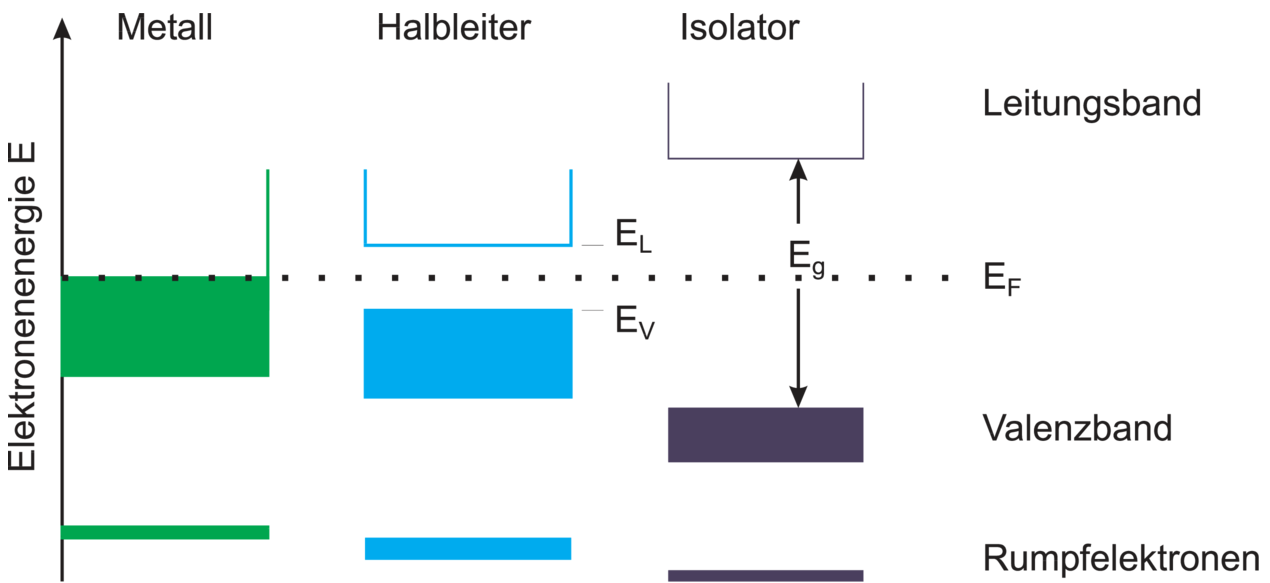
\includegraphics[scale=0.4]{pictures/Bandstrukturen.png}
    \caption{\cite{Halbleiter-Grundlagen}}
\end{figure}

\subsubsection*{Konzept der effektiven Masse von freien Ladungsträgern in Festkörpern}
\begin{itemize}
\item effektive Masse ist ein Maß für die WW des e an das Kristallfeld
\item große effektive Masse \iff starke Kopplung an Kristallfeld \to das Potential ist schwach gekrümmt
\item mathematisch: 
    Taylorreihe von Energie
    \begin{equation*}
        \epsilon(\vec{k})=\epsilon(0)+\frac{1}{2}\sum_{i=1}^3\left(\frac{\partial \epsilon^2}{\partial k_i^2}\right)+O(k^4)
    \end{equation*}
    quadratischer Ausdruck unterscheidet sich in Ordnung O(k²) durch die effektive Masse
    vom Potential eines freien Teilchens.
    \begin{equation*}
        \epsilon_{V=0}=\frac{\hbar^2 k^2}{2m}
    \end{equation*}
    Die effektive Masse ist also 
    \begin{equation*}
        m_i^*=\frac{\hbar²}{\left(\frac{\partial \epsilon^2}{\partial k_i^2}\right)_{k=0}}.
    \end{equation*}
\end{itemize}

\subsection{Dotierung von Halbleitern}
\subsubsection*{Warum ist Dotierung nötig?}
\begin{itemize}
    \item Dotierung erhöht die Anzahl an elektrischen Ladungsträgern
        \to n-Dotierung erzeugt Erzeugt ein Elektron im Valenzband 
        \to p-Dotierung erzeugt ein Loch im Leitungsband 
    \item Leitfähigkeit des Halbleiters kann angepasst werden
\end{itemize}

\subsubsection*{Rolle der Donatoren und Akzeptoren, ihre Energieniveaus im Banddiagramm}
\begin{itemize}
    \item Donatoren besitzen ein Valenzelektron mehr als Halbleiter-Material
        \to n-Dotierung
        \to senkt Leitungsband
    \item Akzeptoren besitzen ein Valenzelektron weniger als Halbleiter-Material
        \to p-Dotierung 
        \to erhöht Valenzband
\end{itemize}
\begin{figure}[H]
    \centering
    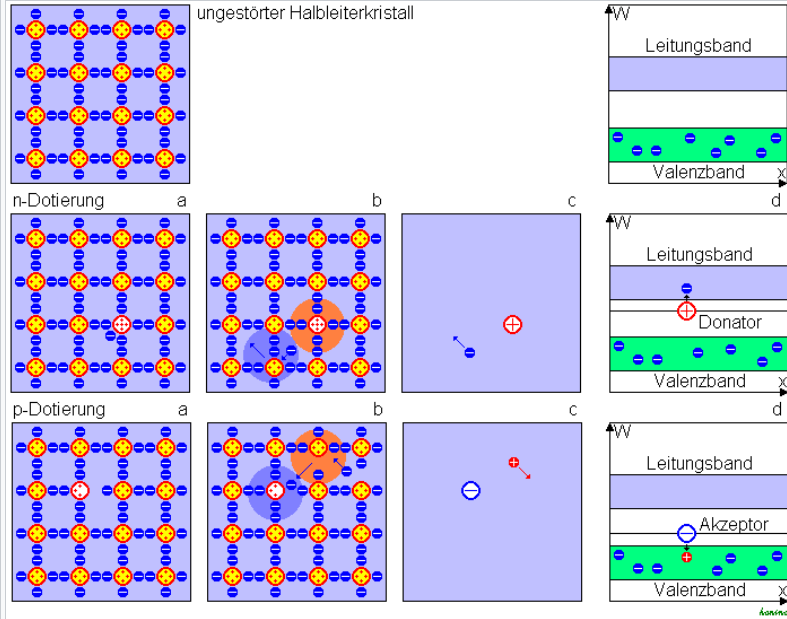
\includegraphics[scale=0.5]{pictures/Dotierung.png}
    \caption{\cite{Dotierung}}
\end{figure}

\subsection{Faraday-Effek}
\subsubsection*{Definition des Effekts der Faraday-Rotation}
\begin{itemize}
    \item linear polarisierte Welle = Superposition zweier zirkular polarisierter Wellen (gleiche Frequenz, entgegengesetzer Umlaufsinn)
        \begin{equation*}
            E(z)=\frac{1}{2}(E_R(z)+E_L(z))    
        \end{equation*}
    \item wenn Ausbreitungsrichtung parallel zum B-Feld unterscheiden sich (meist) die Brechungsindizes $n$
        \to unterschiedliche Wellenlängen
        \iff Polarisationsebene verdreht sich pro Schwingungsdauer $T$ um 
        \begin{equation*}
            \Delta\beta=\pi\cdot\left(\frac{n_{rechts}}{n_{links}}-1\right)
        \end{equation*} 
    \item Grund: induzierte elektrische Dipolmomente innerhalb des Materials erzeugen eine Polarisation des Materials
        \begin{equation*}
            \vec{P}=\epsilon_0 \chi\vec{E}
        \end{equation*}
        wobei $\chi$ eine 3x3-Matrix ist.
    \item Doppebrechung für 
        \begin{equation*}
            \chi = \left[ 
            \begin{array}{ccc}
                \chi_{xx}          & +i\chi_{xy} & 0         \\ 
                -i\chi_{xy}   & \chi_{yy}        & 0         \\
                0                  & 0                & \chi_{zz} \\ 
            \end{array}
            \right]
        \end{equation*}
\end{itemize}

\subsubsection*{Phänomenologische Beschreibung}
\begin{itemize}
    \item zikulare Doppelbrechung:
        Fähigkeit eines Kristalls, die Polarisationsebene eines linear polarisierten Lichtstrahls bei der Transmission zu drehen
        \begin{figure}[H]
            \centering
            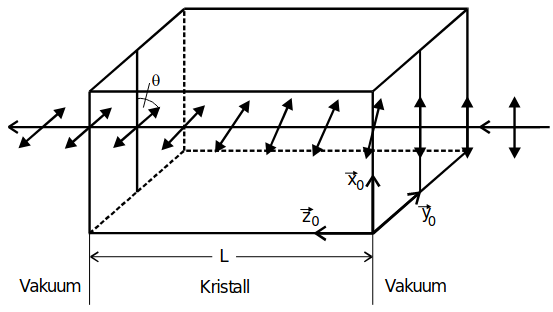
\includegraphics[scale=0.5]{pictures/Doppelbrechung.png}
            \caption{\cite{Anhang}}
        \end{figure}
        \to optisch aktive Materie
    \item durch anlegen eines Magnetfeldes wird optisch inaktive Materie doppelbrechend
        \to Symmetrie des Kristalls wird gebrochen
\end{itemize}

\subsection{Bestimmung der effektiven Masse von Ladungsträgern mittels des Faraday-Effekts}
\subsubsection*{Modelle und Ansatz}
\begin{itemize}
    \item messe Faraday-Effekt für dotierte und nicht dotierte Polarisationsebene
        \to Differenz der Probe ist der Einfluss der Leitungselektronen
        \begin{equation*}
            \theta_{frei}=\frac{e_0^3}{8\pi^2\epsilon_0c^3}\frac{1}{(m^*)^2}\lambda^2\frac{NB}{n}
        \end{equation*}
        \begin{itemize}
            \item $\theta_{frei}=\theta_{dotierte}-\theta_{rein}$: Faraday-Rotation
            \item $e_0$: Elemenatarladung
            \item $\epsilon_0$: Influenzkonstante
            \item $c$: Lichtgeschwindigkeit
            \item $m^*$: effektive Masse des Elektrons 
            \item $\lambda$: Wellenlänge des Lichts 
            \item $N$: Donatorkonzentration
            \item $B$: Magnetfeldstärke
            \item $L$: Probendicke
            \item $n$: Brechungsindex
        \end{itemize}
\end{itemize}

\subsubsection*{Wie beeinflussen Magnetfelder freie Elektronen?}
\begin{itemize}
    \item je nach Spin wird Energie um $\epsilon_{Zeeman}$ erhöht oder erniedrigt
        \to Fermienergie $\epsilon_F$ bleibt gleich
        \iff in den Bandhälften befindet sich eine unterschiedliche Anzahl an e 
\end{itemize}
\begin{figure}[H]
    \centering
    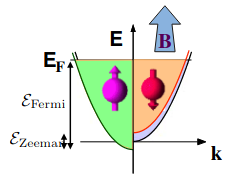
\includegraphics[scale=0.8]{pictures/magnetfeld_freieElektronen.png}
    \\caption{\cite{Magnetismus}}
\end{figure}

\subsection{Detektionstechnik}
\subsubsection*{Warum ermöglicht die Modulation des Lichts in Kombination mit selektiver Verstärkung eine Unterdrückung des Signalrauschens?} %???
\begin{itemize}
    \item Signalrauschen entsteht durch Photowiderstände (Dunkelrate)
    \item Sektorscheibe zerhackt Lichtsignale
        \to Lichtimpulse und Dunkelheit wechseln sich Abgabe
        \iff Impusle können besser vom Untergrund getrennt werden
    \item Selektivverstärker wird als Nulldetektor verwendet
        \to vergleicht die Signalspannungen beider Photowiderstände miteinander
\end{itemize}


\subsection{Alternativer Ansatz zur Detektion} 
\subsection*{Was ist der Hauptvorteil der balancierten Detektion mit zwei Photodetektoren?} %???
\begin{itemize}
    \item Zweistrahlverfahren für hohe Winkelauflösung
\end{itemize}
\subsection*{Kann man die Faraday-Rotation auch mit nur einem Detektor messen?} %???
\begin{itemize}
    \item Ja
    \item schicke linear polarisiertes Licht durch Polfilter
        \to bei richtiger Einstellung sollte kein Licht durch den Polfilter gelangen
    \item Schalte B-Feld an 
        \to Polfilter muss nun um Winkel $theta$ gedreht werden, bis die Intensität hinter dem Polfilter wieder auf 0 absinkt
    \item hinter dem Filter wird also nur ein Photowiderstand benötigt 
\end{itemize}